\documentclass[12pt]{beamer}
\newenvironment{ConCodigo}[1]
  {\begin{frame}[fragile,environment=ConCodigo]{#1}}
  {\end{frame}}
\graphicspath{{Imagenes/}{../Imagenes/}}
\usepackage[utf8]{inputenc}
\usepackage[spanish]{babel}
\usepackage{hyperref}
\usepackage{etex}
\reserveinserts{28}
\usepackage{amsmath}
\usepackage{amsthm}
\usepackage{mathtools}
\usepackage{multicol}
\usepackage{multirow}
\usepackage{tabulary}
\usepackage{booktabs}
\usepackage{nccmath}
\usepackage{biblatex}
\usepackage{epstopdf}
\usepackage{graphicx}
%\usepackage{enumitem,xcolor}
\usepackage{siunitx}
\sisetup{scientific-notation=true}
%\usepackage{fontspec}
\usepackage{lmodern}
\usepackage{float}
\usepackage[format=hang, font=footnotesize, labelformat=parens]{caption}
\usepackage[autostyle,spanish=mexican]{csquotes}
\usepackage{standalone}
\usepackage{blkarray}
\usepackage{algorithm}
\usepackage{algorithmic}
\usepackage{tikz}
\usepackage[siunitx]{circuitikz}
\usetikzlibrary{arrows,patterns,shapes}
\usetikzlibrary{decorations.markings}
\usetikzlibrary{arrows}
\usepackage{color}
\usepackage{xcolor}
%\usepackage{beton}
%\usepackage{euler}
%\usepackage[T1]{fontenc}
\usepackage[sfdefault]{roboto}  %% Option 'sfdefault' only if the base font of the document is to be sans serif
\usepackage[T1]{fontenc}
\renewcommand*\familydefault{\sfdefault}
\DeclareGraphicsExtensions{.pdf,.png,.jpg}
\usepackage{hyperref}
\renewcommand {\arraystretch}{1.5}
\newcommand{\python}{\texttt{python}}
\usefonttheme[onlymath]{serif}
\setbeamertemplate{navigation symbols}{}
\usetikzlibrary{patterns}
\usetikzlibrary{decorations.markings}
\tikzstyle{every picture}+=[remember picture,baseline]
%\tikzstyle{every node}+=[inner sep=0pt,anchor=base,
%minimum width=2.2cm,align=center,text depth=.15ex,outer sep=1.5pt]
%\tikzstyle{every path}+=[thick, rounded corners]
\setbeamertemplate{caption}[numbered]
\newcommand{\ptm}{\fontfamily{ptm}\selectfont}
%Se usa la plantilla Warsaw modificada con spruce
\mode<presentation>
{
  \usetheme{Warsaw}
  \setbeamertemplate{headline}{}
  \useoutertheme{default}
  \usecolortheme{seahorse}
  \setbeamercovered{invisible}
}
% \AtBeginSection[]
% {
% \begin{frame}<beamer>{Contenido}
% \normalfont\mdseries
% \tableofcontents[currentsection]
% \end{frame}
%}

\usepackage{listings}
\lstset{ %
language=Python,                % choose the language of the code
basicstyle=\small,       % the size of the fonts that are used for the code
numbers=left,                   % where to put the line-numbers
numberstyle=\footnotesize,      % the size of the fonts that are used for the line-numbers
stepnumber=1,                   % the step between two line-numbers. If it is 1 each line will be numbered
numbersep=5pt,                  % how far the line-numbers are from the code
backgroundcolor=\color{white},  % choose the background color. You must add \usepackage{color}
showspaces=false,               % show spaces adding particular underscores
showstringspaces=false,         % underline spaces within strings
showtabs=false,                 % show tabs within strings adding particular underscores
frame=single,   		% adds a frame around the code
tabsize=4,  		% sets default tabsize to 2 spaces
captionpos=b,   		% sets the caption-position to bottom
breaklines=true,    	% sets automatic line breaking
breakatwhitespace=false,    % sets if automatic breaks should only happen at whitespace
escapeinside={\#}{)}          % if you want to add a comment within your code
}

\title{Tema 1 - Representación de números de punto flotante}
\subtitle{Curso de Física Computacional}
\author[]{M. en C. Gustavo Contreras Mayén}
\date{}
\begin{document}
\maketitle
\fontsize{14}{14}\selectfont
\spanishdecimal{.}
\begin{frame}{Contenido}
\tableofcontents[pausesections]
\end{frame}
\section{Representación de números de punto flotante}
\subsection{Qué es lo que pasa?}
\begin{frame}[fragile]
\frametitle{¿Qué es lo que pasa?}
Realiza la siguiente operación en Python:
\\
\bigskip
\texttt{>>> 1 - 0.9 - 0.1}
\\
\medskip
\visible<2->{\textcolor{blue}{\texttt{-2.7755575615628914e-17}}}
\visible<3->{\begin{alertblock}{Pregunta}
¿Por qué el resultado que esperamos no es cero?
\end{alertblock}}
\end{frame}
\begin{frame}[fragile]
\frametitle{Considera el siguiente código}
\begin{lstlisting}
suma = 1
for i in range(1,1000001):
    suma = suma+0.0000001
print suma
\end{lstlisting}
¿Cuál es el resultado que nos devuelve el programa?
\\
\bigskip
\pause
\textcolor{blue}{\texttt{1.10000000006}}
\\
\medskip
\pause
\begin{alertblock}{Pregunta}
\textcolor{red}{¿En dónde está el error?}
\end{alertblock}
\end{frame}
\begin{frame}
Para dar respuesta a las preguntas, tendremos que ahondar en la manera en que se representan los números en una computadora.
\end{frame}
\section{Código binario}
\begin{frame}
\frametitle{Código binario}
La forma de almacenar un número en una computadora es mediante el sistema binario (código binario), es decir, sólo utiliza el $0$ y el $1$ para representar cualquier número.
\\
\medskip
Según sea el diseño de la arquitectura y el hardware de una computadora, será la precisión con la que se represente un número. Por ejemplo, para una computadora que utiliza 8 bytes, es decir, 64 bits para representar un entero, el primer bit lo utiliza para el signo y los restantes 63 para el número, así el máximo valor que se puede representar será
\[ \sum_{k=0}^{62} 2^{k} \]
\end{frame}
\begin{frame}
El formato para la representación de un número real en una computadora depende del diseño de
hardware y software. El formato común es el de \emph{punto flotante}, donde se le asignan ciertos bits para guardar el exponente y el resto para la mantisa.
\\
\medskip
La razón más común de los errores en una computadora se atribuyen al error de representar un número real mediante un número limitado de bits, comúnmente se denominan errores de redondeo al guardar un número en la memoria.
\end{frame}
\begin{frame}
El épsilon, $\epsilon$, de la computadora es lo que determina la precisión con la que se representa un número, como ya vimos, se define como el tamaño del intervalo entre $1$ y el siguiente número mayor que $1$ distinguible de 1. Esto significa que ningún número entre $1$ y  $1 + \epsilon$ se puede representar en la computadora.
\\
\medskip
Por ejemplo, cualquier número $1 + \alpha$ se redondea a $1$ si $0 <\alpha <\epsilon/2$, o se redondea a $1 + \epsilon$ si $\epsilon/2 \leq \alpha$.
\\
\medskip
Por lo que se puede considerar que $\epsilon/2$ es el máximo error posible de redondeo para $1$. En otras palabras, cuando se halla $1.0$ en la memoria de la computadora, el valor original pudo estar entre $1-\epsilon/2 < x < 1 + \epsilon/2$.
\end{frame}
\begin{frame}
Finalmente se puede concluir que el error de redondeo implicado al guardar cualquier número real
$R$ en la memoria de una computadora, es aproximadamente igual a $\epsilon R / 2$, si el número se redondea por exceso y $\epsilon R$ si se redondea por defecto.
\end{frame}
\begin{frame}
\frametitle{Operaciones aritméticas en binario}
Las cuatro operaciones aritméticas básicas: suma, resta, multiplicación y división en notación binaria presentan dos tipos de situaciones en los que aparecen muchos errores de redondeo:
\begin{itemize}
\item Cuando se suma o se resta un número muy pequeño con uno muy grande.
\item Cuando se divide entre un número pequeño o se multiplica por un número muy grande.
\end{itemize}
\end{frame}
\begin{frame}
\frametitle{Ejemplo de suma binaria}
Para ejemplificar cómo surgen los errores de redondeo se considera el cálculo de $1$ y $0.00001$ con una mantisa de $24$ bits; por tanto, en base 2 se tiene que:
\begin{eqnarray*}
(1)_{10} &= (0.1000 0000 0000 0000 0000 0000)_{2} \times 2^{1} \\
(0.00001)_{10} &= 0.1010 0111 1100 0101 1010 1100)_{2} \times 2^{-16}
\end{eqnarray*}
La suma de estos dos números es:
\[ \begin{split}
(1)_{10} + (0.00001)_{10}  = (0.1000 0000 0000 0000 0101 0011 \\
 \mathbf{1110 0010 1101 0110 0})_{2} \times 2^{1}
\end{split} \]
\end{frame}
\begin{frame}
\[ \begin{split}
(1)_{10} + (0.00001)_{10}  = (0.1000 0000 0000 0000 0101 0011 \\
 \mathbf{1110 0010 1101 0110 0})_{2} \times 2^{1}
\end{split} \]
Como se considera una mantisa de sólo $24$ bits, se redondea a partir de los números en negrita. Por tanto, el resultado de esta suma, se almacena en la memoria como:
\[ (1)_{10} + (0.00001)_{10}  = (0.1000 0000 0000 0000 0101 0011)_{2} \times 2^{1} \]
que equivale a $(1.0000 1001 36)_{10}$
\end{frame}
\begin{frame}
\frametitle{Conclusión}
Así, siempre que se sumen $1$ y $0.00001$, el resultado agrega $0.0000000136$ como error. En las operaciones fundamentales, algunas cantidades se redondean por exceso y otros por defecto. La pérdida y ganancia se conoce como error de redondeo.
\end{frame}
\section{Números en representación de punto flotante}
\begin{frame}
\frametitle{Números en representación de punto flotante}
La forma estándar de representar un número real en forma decimal es con una parte entera, un punto decimal y una parte fraccionaria, por ejemplo $45.67432$ o $0.00012534$. Otra forma estándar, llamada \emph{notación científica normalizada}, en la cual la parte entera es cero y se obtiene al multiplicar por una potencia adecuada de $10$.
\\
\medskip
Se tiene que $45.67432$ se puede representar en notación científica normalizada como
$0.4567432 \times 10^{2}$ y $0.0012534$ como $0.12534 \times 10^{-2}$.
\end{frame}
\begin{frame}
\frametitle{Representación de punto flotante}
En notación científica, un número se representa por una fracción multiplicada por una potencia de $10$ y el primer número a la derecha del punto decimal es diferente de cero. En computación a la notación científica normalizada se le llama \emph{representación de punto flotante}.
\end{frame}
\begin{frame}
Un sistema computacional representa a los números en punto flotante con las limitaciones que impone una longitud finita de palabra. Una computadora puede tener una longitud de palabra de $64$ bits (dígitos binarios) la cual puede representar números binarios en la forma
\[ x = \pm q \times 2^{m}\]
donde
\begin{itemize}
\item el signo de $x$ ocupa $1$ bit.
\item el signo de $m$ ocupa $1$ bit.
\item el entero $\vert m \vert$ ocupa $10$ bits.
\item el número $q$ ocupa $52$ bits.
\end{itemize}
Al número $q$ se le denomina \emph{mantisa} y al número $m$ se le llama \emph{exponente}. Si se supone que $m$ se puede representar con a lo más $10$ bits entonces el máximo valor de $m$ que se puede representar es $2^{10} – 1 = 1 023$.
\end{frame}
\begin{frame}
\frametitle{Números de máquina}
Los números reales representables en una computadora se llaman\emph{números de máquina}. Para poder representar un número 
\[ x = 0.d_{1} d_{2} d_{3} \ldots \times 10^{m} \]
como número de máquina, denotado por $fl(x)$, se obtiene cortando la mantisa de $x$ en $k$ cifras.
Existen dos formas de efectuar ese corte:
\begin{enumerate}
\item La primera es simplemente eliminando los dígitos a partir de $d_{k+1}$. Esta forma recibe el nombre de truncamiento.
\item La segunda forma es determinar a $d_{k}$ a partir de $d_{k+1}$, si $d_{k+1} < 5$, $d_{k}$ queda sin cambio. En caso contrario, aumentamos en uno $d_{k}$, esto se conoce como redondeo.
\end{enumerate}
\end{frame}
\section{Propagación de errores}
\begin{frame}
\frametitle{Propagación de errores}
Para investigar la propagación del error en cálculos sucesivos se consideran dos números $p$ y $q$ junto con sus aproximaciones  $\widehat{p}$ y  $\widehat{q}$ con errores $\epsilon_{p}$ y $\epsilon_{q}$, respectivamente. Entonces
\[ p+q = (\widehat{p} + \epsilon_{p}) + (\widehat{q}+ \epsilon_{q}) = (\widehat{p}+\widehat{q})+ (\epsilon_{p} + \epsilon_{q}) \]
por lo que el error de la suma, es la suma de los errores y el error relativo está dado por:
\[ \dfrac{(p+q)-(\widehat{p}+\widehat{q})}{(p+q)} = \dfrac{\epsilon_{p} + \epsilon_{q}}{p+q}\]
\end{frame}
\begin{frame}
Para la multiplicación se tiene que:
\[ pq = (\widehat{p}+\epsilon_{p})(\widehat{q}+\epsilon_{q}) = \widehat{p}\widehat{q}+\widehat{p}\epsilon_{q}+\widehat{q}\epsilon_{p} + (\epsilon_{p} + \epsilon_{q})\]
Por lo que si $\vert p \vert$, $\vert q \vert$ $>1$, los términos $\widehat{p}\epsilon_{q}$ y $\widehat{q} \epsilon_{p}$ muestran un aumento en los errores originales.
\end{frame}
\begin{frame}
Para tener una mejor visión de la multiplicación, se calcula el error relativo, bajo las suposiciones: $p,q \neq 0, \frac{\widehat{p}}{p} \simeq 1 , \frac{\widehat{q}}{q} \simeq 1, \dfrac{\epsilon_{p}}{p} \dfrac{\epsilon_{q}}{q} = E_{p} E_{q} \simeq 0$. Se tiene que
\[ \begin{split} \dfrac{pq-\widehat{p}\widehat{q}}{pq} = (\widehat{p}+\epsilon_{p}+\epsilon_{p})(\widehat{q}+\epsilon_{q}) = \dfrac{\epsilon_{q}}{q}+\dfrac{\epsilon_{p}}{p}+ E_{p}E_{q} \simeq \\
\simeq \dfrac{\epsilon_{q}}{q}+\dfrac{\epsilon_{p}}{p} = E_{p}+E{q}
\end{split}  \]
El error relativo en el producto es aproximadamente la suma de las razones entre los errores y las aproximaciones.
\end{frame}
%\section{Representación de números enteros}
%\subsection{Signo y Magnitud}
%\begin{frame}[fragile]
%\frametitle{Signo y Magnitud}
%En la representación de un número entero en \textit{Signo y Magnitud}, de los \textbf{n} bits de dicha representación, el más significativo representa el signo de la misma representación, por lo que se llama \textit{bit de signo}.
%\\
%\bigskip
%El resto de los bits representan la magnitud.
%\[ N_{SM} = a_{n-1} a_{n-2} \ldots a_{1} a_{0}\]
%donde $a_{n-1}$ representa el signo del número y el resto de los bits, la magnitud del mismo:
%\end{frame}
%\begin{frame}[fragile]
%\frametitle{Representación de Signo y Magnitud}
%\begin{center}
%\begin{tikzpicture}[scale=0.8]
%\draw (0,0) rectangle (1.5,1.5);
%\draw (0,0) rectangle (3,1.5);
%\draw (0,0) rectangle (4.5,1.5);
%\draw (0,0) rectangle (6,1.5);
%\draw (0,0) rectangle (7.5,1.5);
%\draw (0,0) rectangle (9,1.5);
%\draw (0,0) rectangle (10.5,1.5);
%\draw [font=\small] (0.5,1.7) node {$a_{n-1}$};
%\draw [font=\small] (2.1,1.7) node {$a_{n-2}$};
%\draw [font=\small] (3.7,1.7) node {$a_{n-3}$};
%\draw [font=\small] (6.5,1.7) node {$\ldots$};
%\draw [font=\small] (8.3,1.7) node {$a_{1}$};
%\draw [font=\small] (9.9,1.7) node {$a_{0}$};
%\draw [font=\small] (0.5,-0.3) node {bit de signo};
%\draw [font=\small] (6.5,-0.3) node {bits de la magnitud};
%\end{tikzpicture}
%\end{center}
%Cuando se quiera representar el signo del número negativo, el bit de signo valdrá $\mathbf{1}$, siendo $\mathbf{0}$ cuando el número es positivo.
%\end{frame}
%\begin{frame}
%\frametitle{Rango de operación en Signo Magnitud}
%El rango de representación de este sistema es el siguiente:
%\[ \left( -2^{n-1} + 1 \right)_{10} \leq x \leq \left(2^{n-1} -1 \right)_{10} \]
%\end{frame}
%\begin{frame}[fragile]
%\frametitle{Ejercicio 1}
%En SM para $\mathbf{n}=8$, el bit $a_{7}$ representa el signo del número y es resto de bits, la magnitud del mismo:
%\begin{center}
%\begin{tikzpicture}[scale=0.8]
%\draw (0,0) rectangle (1.5,1.5);
%\draw (0,0) rectangle (3,1.5);
%\draw (0,0) rectangle (4.5,1.5);
%\draw (0,0) rectangle (6,1.5);
%\draw (0,0) rectangle (7.5,1.5);
%\draw (0,0) rectangle (9,1.5);
%\draw (0,0) rectangle (10.5,1.5);
%\draw [font=\small] (0.5,1.7) node {$a_{7}$};
%\draw [font=\small] (2.1,1.7) node {$a_{6}$};
%\draw [font=\small] (3.7,1.7) node {$a_{5}$};
%\draw [font=\small] (6.5,1.7) node {$\ldots$};
%\draw [font=\small] (8.3,1.7) node {$a_{1}$};
%\draw [font=\small] (9.9,1.7) node {$a_{0}$};
%\draw [font=\small] (0.5,-0.3) node {bit de signo};
%\draw [font=\small] (7.5,-0.3) node {bits de la magnitud};
%\end{tikzpicture}
%\end{center}
%\pause
%Su rango de representación es:
%\begin{eqnarray*}
%\left( -2^{8-1} + 1\right)_{10} & \leq & x \leq \left( 2^{8-1} - 1\right)_{10} \\
%\left( 2^{7}+1 \right) & \leq & x \leq \left( 2^{7} -1 \right)_{10} \\
%(-128+1)_{10} & \leq & x \leq (128-1)_{10} \\
%-127_{10} & \leq & x \leq 127_{10}
%\end{eqnarray*}
%Por tanto, se pueden representar $2^{8}-1=255$ números enteros.
%\end{frame}
%\begin{frame}[fragile]
%\frametitle{Ejercicio 2}
%Expresa en SM, para $\mathbf{n=8}$, el número $23_{10}$
%\begin{center}
%	\begin{tikzpicture}[scale=0.8,font=\small]
%		\draw (0,0) rectangle (1.5,1.5);
%		\draw (0,0) rectangle (3,1.5);
%		\draw (0,0) rectangle (4.5,1.5);
%		\draw (0,0) rectangle (6,1.5);
%		\draw (0,0) rectangle (7.5,1.5);
%		\draw (0,0) rectangle (9,1.5);
%		\draw (0,0) rectangle (10.5,1.5);
%		\draw (0,0) rectangle (12,1.5);
%		\draw (-0.75,0.75) node {$23_{10} =$};
%		\draw (0.5,1.7) node {$a_{7}$};
%		\draw (2.1,1.7) node {$a_{6}$};
%		\draw (3.7,1.7) node {$a_{5}$};
%		\draw (5.3,1.7) node {$a_{4}$};
%		\draw (6.5,1.7) node {$a_{3}$};
%		\draw (8.3,1.7) node {$a_{2}$};
%		\draw (9.9,1.7) node {$a_{1}$};
%		\draw (11.5,1.7) node {$a_{0}$};
%		\draw (0.5,-0.3) node {bit de signo};
%		\draw (7.5,-0.3) node {bits de la magnitud};
%		\pause;
%		\draw [font=\large](0.75,0.75) node {$\mathbf{0}$};
%		\draw [font=\large](2.25,0.75) node {$\mathbf{0}$};
%		\draw [font=\large](3.75,0.75) node {$\mathbf{0}$};
%		\draw [font=\large](5.25,0.75) node {$\mathbf{1}$};
%		\draw [font=\large](6.75,0.75) node {$\mathbf{0}$};
%		\draw [font=\large](8.25,0.75) node {$\mathbf{1}$};
%		\draw [font=\large](9.75,0.75) node {$\mathbf{1}$};
%		\draw [font=\large](11.25,0.75) node {$\mathbf{1}$};
%	\end{tikzpicture}
%\end{center}
%\pause
%De tal manera que
%\[ \mathbf{23_{10} = 00010111_{SM}}\]
%\end{frame}
%\begin{frame}[fragile]
%\frametitle{Ejercicio 3}
%Expresa en SM para $\mathbf{n=8}$ el número $-23_{10}$
%\begin{center}
%	\begin{tikzpicture}[scale=0.8,font=\small]
%		\draw (0,0) rectangle (1.5,1.5);
%		\draw (0,0) rectangle (3,1.5);
%		\draw (0,0) rectangle (4.5,1.5);
%		\draw (0,0) rectangle (6,1.5);
%		\draw (0,0) rectangle (7.5,1.5);
%		\draw (0,0) rectangle (9,1.5);
%		\draw (0,0) rectangle (10.5,1.5);
%		\draw (0,0) rectangle (12,1.5);
%		\draw (-0.75,0.75) node {$23_{10} =$};
%		\draw (0.5,1.7) node {$a_{7}$};
%		\draw (2.1,1.7) node {$a_{6}$};
%		\draw (3.7,1.7) node {$a_{5}$};
%		\draw (5.3,1.7) node {$a_{4}$};
%		\draw (6.5,1.7) node {$a_{3}$};
%		\draw (8.3,1.7) node {$a_{2}$};
%		\draw (9.9,1.7) node {$a_{1}$};
%		\draw (11.5,1.7) node {$a_{0}$};
%		\draw (0.5,-0.3) node {bit de signo};
%		\draw (7.5,-0.3) node {bits de la magnitud};
%		\pause;
%		\draw [font=\large](0.75,0.75) node {$\mathbf{1}$};
%		\draw [font=\large](2.25,0.75) node {$\mathbf{0}$};
%		\draw [font=\large](3.75,0.75) node {$\mathbf{0}$};
%		\draw [font=\large](5.25,0.75) node {$\mathbf{1}$};
%		\draw [font=\large](6.75,0.75) node {$\mathbf{0}$};
%		\draw [font=\large](8.25,0.75) node {$\mathbf{1}$};
%		\draw [font=\large](9.75,0.75) node {$\mathbf{1}$};
%		\draw [font=\large](11.25,0.75) node {$\mathbf{1}$};
%	\end{tikzpicture}
%\end{center}
%\pause
%Por tanto:
%\[ \mathbf{-23_{10} = 1001011_{SM}} \]
%\end{frame}
%\subsection{Exceso a $2^{n-1}$}
%\begin{frame}[fragile]
%\frametitle{¿Qué es el Exceso a $2^{n-1}$?}
%En Exceso a $2^{n-1}$ tenemos que si se dispone de \textbf{n} bits para representar a un número entero (\textbf{N}) positivo o negativo, dicho número se representa como $N + 2^{n-1}$, por lo que:
%\[ N_{Ex} = N + 2^{n-1} \]
%\end{frame}
%\begin{frame}[fragile]
%\frametitle{Ejemplo}
%En Exceso a $2^{n-1}$ para $n=16$, el número positivo $9503_{10}$ se presenta como:
%\[ \begin{split}
%9503_{10} =& (9503_{10} + (2^{16-1})_{10}) \\
%\uncover<2->{ =& (9503_{10} + (2^{15})_{10})} \\
%\uncover<3->{ =& (9503_{10} + 32768_{10})} \\
%\uncover<4->{ =& (42271_{10})} \\
%\uncover<5->{ =& (1010010100011111_{2})} \\
%\uncover<6->{ =& 1010010100011111_{\text{Exp a } 32768}}
%\end{split} \]
%\end{frame}
%\subsection{Estándar IEEE 754}
%\begin{frame}
%\frametitle{El Estándar IEE 754}
%El estándar IEEE 754 establece dos formatos básicos para representar a los números reales en la computadora:
%\begin{itemize}
%\item de precisión simple.
%\item de precisión doble.
%\end{itemize}
%\end{frame}
%\subsubsection{Precisión simple}
%\begin{frame}[fragile]
%\frametitle{Precisión simple}
%Cuando se representa un número real en precisión simple, se usan 32 bits (4 bytes) de la siguiente manera:
%\begin{enumerate}
%\item 1 bit para el signo (\textbf{s}) de número.
%\item 8 bits para el exponente (\textbf{exp})
%\item 23 bits para la mantisa (\textbf{m}) que se distribuyen de la siguiente forma:
%\end{enumerate}
%\begin{tikzpicture}[scale=0.8]
%\draw (0,0) rectangle (1,1.5);
%\draw [font=\small] (0.5,1.7) node {31};
%\draw [font=\small\bfseries] (0.5,0.75) node {s};
%\draw [font=\small] (0.5,-0.25) node {signo};
%\draw (0,0) rectangle (4,1.5);
%\draw [font=\small] (1.4,1.7) node {30};
%\draw [font=\small\bfseries] (2.5,0.75) node {exp};
%\draw [font=\small] (2.5,-0.25) node {exponente};
%\draw [font=\small] (2.55,1.7) node {...};
%\draw [font=\small] (3.8,1.7) node {23};
%\draw (0,0) rectangle (14,1.5);
%\draw [font=\small] (4.4,1.7) node {22};
%\draw [font=\small\bfseries] (9,0.75) node {m};
%\draw [font=\small] (9,-0.25) node {mantisa};
%\draw [font=\small] (9,1.7) node {...};
%\draw [font=\small] (13.8,1.7) node {0};
%\end{tikzpicture}
%\end{frame}
%\begin{frame}
%El exponente se suele representar en notación \textit{Exceso a $2^{n-1}$}, mientras que para la mantisa, normalmente se usa el Signo y Magnitud.
%\\
%\bigskip
%La mantisa se suele normalizar colocando el punto decimal a la derecha del bit más significativo.
%\end{frame}
%\begin{frame}
%\frametitle{Ejemplo}
%Para escribir el número
%\[101110.010101110100001111100001111100010011_{2}\]
%en el estándar IEEE 754 con precisión simple, exponente en Exceso a $2^{n-1}$ y mantisa en Signo y Magnitud, lo primero que que hay que hacer es normalizarlo:
%\pause
%\[1.01110010101110100001111100001111100010011_{2} \times 2^{5}\]
%\end{frame}
%\begin{frame}
%El exponente en Exceso a $2^{n-1}-1$ será:
%\[ \begin{split}
%5_{10} + (2^{8-1} - 1)_{10} = & 5_{10} + (27 - 1)_{10} = {} \\
%{} = & 5_{10} + (128 - 1)_{10} = {} \\
%{} = & 132_{10} = {} \\
%{} = & 10000100_{\text{Exp. a } 127} 
%\end{split} \]
%\end{frame}
%\begin{frame}
%Tomamos de la mantisa los 23 bits más significativos:
%\[1.01111001010111000000111 \]
%El resto de los bits no se puede representar ya que no caben en la mantisa.
%\\
%\bigskip
%Cuando la mantisa se normaliza dejando el punto decimal a la derecha del bit más significativo, dicho bit siempre vale \textbf{1}, por lo que se puede prescindir de él y tomar agregar en su lugar otro bit, por lo que aumenta la precisión del número representado:
%\pause
%\[01110010101110000001111 \]
%\end{frame}
%\begin{frame}[fragile]
%Al bit omitido se le llama \textit{bit implícito}. Por otra lado, el bit del signo vale \textbf{0}, ya que es un número positivo, por tanto, el número se puede representar como:
%\begin{tikzpicture}[scale=0.8]
%\draw (0,0) rectangle (1,1.5);
%\draw [font=\small] (0.5,1.7) node {31};
%\draw [font=\small\bfseries] (0.5,0.75) node {0};
%\draw [font=\small] (0.5,-0.25) node {signo};
%\draw (0,0) rectangle (4,1.5);
%\draw [font=\small] (1.4,1.7) node {30};
%\draw [font=\small\bfseries] (2.5,0.75) node {10000100};
%\draw [font=\small] (2.5,-0.25) node {exponente};
%\draw [font=\small] (2.55,1.7) node {...};
%\draw [font=\small] (3.8,1.7) node {23};
%\draw (0,0) rectangle (14,1.5);
%\draw [font=\small] (4.4,1.7) node {22};
%\draw [font=\small\bfseries] (9,0.75) node {01110010101110000001111};
%\draw [font=\small] (9,-0.25) node {mantisa};
%\draw [font=\small] (9,1.7) node {...};
%\draw [font=\small] (13.8,1.7) node {0};
%\end{tikzpicture}
%\end{frame}
%\subsubsection{Precisión doble}
%\begin{frame}[fragile]
%\frametitle{Precisión doble}
%En precisión doble, para escribir un número real, se utilizan 64 bits (8 bytes):
%\begin{enumerate}
%\item  1 bit para el signo (\textbf{s}) del número.
%\item 11 bits para el exponente (\textbf{exp})
%\item 52 bits para la mantisa (\textbf{m}).
%\end{enumerate}
%\begin{tikzpicture}[scale=0.8]
%\draw (0,0) rectangle (1,1.5);
%\draw [font=\small] (0.5,1.7) node {63};
%\draw [font=\small\bfseries] (0.5,0.75) node {s};
%\draw [font=\small] (0.5,-0.25) node {signo};
%\draw (0,0) rectangle (4,1.5);
%\draw [font=\small] (1.4,1.7) node {62};
%\draw [font=\small\bfseries] (2.5,0.75) node {exp};
%\draw [font=\small] (2.5,-0.25) node {exponente};
%\draw [font=\small] (2.55,1.7) node {...};
%\draw [font=\small] (3.8,1.7) node {52};
%\draw (0,0) rectangle (14,1.5);
%\draw [font=\small] (4.4,1.7) node {51};
%\draw [font=\small\bfseries] (9,0.75) node {m};
%\draw [font=\small] (9,-0.25) node {mantisa};
%\draw [font=\small] (9,1.7) node {...};
%\draw [font=\small] (13.8,1.7) node {0};
%\end{tikzpicture}
%\end{frame}
%\begin{frame}[fragile]
%\frametitle{Ejemplo}
%Se quiere expresar el número $19.5625_{10}$ en el estándar IEEE 754 con precisión doble, por lo que tendremos que realizar:
%\begin{enumerate}
%\item Cambiar $19.5625_{10}$ a base 2, iniciando con la parte entera:
%\begin{center}
%\begin{tikzpicture}[overlay]
%\draw [font=\small] (0,0) node {19};
%\draw [thin] (0.4,-0.2) -- (0.4,0.5);
%\draw [thin](0.4,-0.2) -- (1.5,-0.2);
%\draw <1-> [font=\small] (0.8,0) node {2};
%\draw <2-> [font=\small] (0.8,-0.55) node {9};
%\draw <3-> [font=\small\bfseries] (0.1,-0.55) node {1};
%\draw <4-> [->] (-0.1,-0.55) -- (-1.4,-0.55);
%\draw <4-> [font=\small\bfseries] (-2,-0.55) node {$a_{0}=1$};
%\draw <5-> [thin](1,-0.2) -- (1,-0.8);
%\draw <5-> [thin] (1,-0.8) -- (1.7,-0.8);
%\draw <6-> [font=\small] (1.2,-0.55) node {2};
%\draw <7-> [font=\small] (1.2,-1.1) node {4};
%\draw <8-> [font=\small\bfseries] (0.5,-1.1) node {1};
%\draw <9-> [->] (0.3,-1.1) -- (-1.4,-1.1);
%\draw <9-> [font=\small\bfseries] (-2,-1.1) node {$a_{1}=1$};
%\draw <10-> [thin](1.45,-0.8) -- (1.45,-1.35);
%\draw <10-> [thin] (1.45,-1.35) -- (2.1,-1.35);
%\draw <11-> [font=\small] (1.7,-1.1) node {2};
%\draw <12-> [font=\small] (1.7,-1.65) node {2};
%\draw <13-> [font=\small\bfseries] (1,-1.65) node {0};
%\draw <14-> [->] (0.8,-1.65) -- (-1.4,-1.65);
%\draw <14-> [font=\small\bfseries] (-2,-1.65) node {$a_{2}=0$};
%\draw <15-> [thin](1.95,-1.35) -- (1.95,-1.85);
%\draw <15-> [thin] (1.95,-1.85) -- (2.45,-1.85);
%\draw <16-> [font=\small] (2.2,-1.65) node {2};
%\draw <17-> [font=\small\bfseries] (2.2,-2.1) node {1};
%\draw <18-> [font=\small\bfseries] (1.5,-2.1) node {0};
%\draw <19-> [->] (1.3,-2.1) -- (-1.4,-2.1);
%\draw <19-> [font=\small\bfseries] (-2,-2.1) node {$a_{3}=0$};
%\draw <20-> [->] (2.4,-2.1) -- (2.8,-2.1);
%\draw <20-> [font=\small\bfseries] (3.5,-2.1) node {$a_{4}=1$};
%\end{tikzpicture}
%\end{center}
%\end{enumerate}
%\end{frame}
%\begin{frame}[fragile]
%\begin{enumerate}
%\setcounter{enumi}{1}
%\item Ahora la parte fraccionaria
%\end{enumerate}
%\begin{center}
%\begin{tikzpicture}[overlay]
%\draw <1-> (0,0) node {$0.5625 \times 2 = \mathbf{1}.125$};
%\draw <2-> [->] (2.2,0) -- (2.8,0);
%\draw <2-> (3.6,0) node {$a_{.1} = 1$};
%\draw <3-> (0,-0.6) node {$0.125 \times 2 = \mathbf{0}.25$};
%\draw <4-> [->] (2.2,-0.6) -- (2.8,-0.6);
%\draw <4-> (3.6,-0.6) node {$a_{.2} = 0$};
%\draw <5-> (0,-1.2) node {$0.25 \times 2 = \mathbf{0}.5$};
%\draw <6-> [->] (2.2,-1.2) -- (2.8,-1.2);
%\draw <6-> (3.6,-1.2) node {$a_{.3} = 0$};
%\draw <7-> (0,-1.8) node {$0.5 \times 2 = \mathbf{1}$};
%\draw <8-> [->] (2.2,-1.8) -- (2.8,-1.8);
%\draw <8-> (3.6,-1.8) node {$a_{.4} = 1$};
%\end{tikzpicture}
%\end{center}
%\end{frame}
%\begin{frame}
%De modo que el número queda expresado como:
%\[ 19.5625_{10} = 10011.1001_{2}\]
%\pause
%\begin{enumerate}
%\setcounter{enumi}{2}
%\item Se normaliza el número en binario que se obtuvo, dejando el punto decimal a la derecha del bit más significativo:
%\[ 10011.1001_{2} = 1.00111001 \times 2^{4}\]
%\end{enumerate}
%\end{frame}
%\begin{frame}
%\begin{enumerate}
%\setcounter{enumi}{3}
%\item Se escribe el exponente en Exceso a $2^{n-1} -1$
%\[ \begin{split}
%	4_{10} + (2^{11-1} -1)_{10} =& 4_{10} +(2^{10}-1)_{10} \\
%	{} =& 4_{10} + (1024-1)_{10} \\
%	{} =& 1027_{10} \\
%	{} =& 10000000011_{\text{Exp. a } 1023}
%	\end{split}
%	\]
%\item Se deja la mantisa utilizando el bit implícito: se eligen los ocho bits que están a la derecha de la coma $(\mathbf{00111001})$ y el resto de la mantisa se rellena con ceros:
%\[00111001000000 \ldots 000000\]
%\end{enumerate}
%\end{frame}
%\begin{frame}[fragile]
%El número expresado en el estándar IEEE 754 con precisión doble es:
%\\
%\bigskip
%\begin{tikzpicture}[scale=0.8]
%\draw (0,0) rectangle (1,1.5);
%\draw [font=\small] (0.5,1.7) node {63};
%\draw [font=\small\bfseries] (0.5,0.75) node {0};
%\draw [font=\small] (0.5,-0.25) node {signo};
%\draw (0,0) rectangle (4,1.5);
%\draw [font=\small] (1.4,1.7) node {62};
%\draw [font=\small\bfseries] (2.5,0.75) node {10000000011};
%\draw [font=\small] (2.5,-0.25) node {exponente};
%\draw [font=\small] (2.55,1.7) node {...};
%\draw [font=\small] (3.8,1.7) node {52};
%\draw (0,0) rectangle (14,1.5);
%\draw [font=\small] (4.4,1.7) node {51};
%\draw [font=\small\bfseries] (9,0.75) node {00111001000000000000000 \ldots 000000000};
%\draw [font=\small] (9,-0.25) node {mantisa};
%\draw [font=\small] (9,1.7) node {...};
%\draw [font=\small] (13.8,1.7) node {0};
%\end{tikzpicture}
%\end{frame}
\begin{frame}
\subsubsection{Casos especiales del IEEE 754}
\frametitle{Casos especiales del IEEE 754}
Tanto en los tipos de datos de precisión simple como de precisión doble, existen algunos casos especiales que dependen de los valores del signo, del exponente y de la mantisa.
\end{frame}
\begin{frame}
%\fontsize{10}{10}\selectfont
\scalebox{0.8}{
\begin{tabular}{| c | c | c | c |}
\hline
\textbf{Signo (s)} & \textbf{Exponente (exp)} & \textbf{Mantisa (m)} & \textbf{Significado} \\
\hline
\hline

Positivo (0) & \multirow{2}{2.5cm} {Todos unos \\ ($111 \ldots 11$)} & \multirow{2}{2.5cm} {Todos ceros \\ ($000 \ldots 00$)} & \multirow{2}{2.3cm} {Más infinito \\ ($+ \infty$)} \\
 &  &  & \\
\hline
Negativo (1) & \multirow{2}{2.5cm} {Todos unos \\ ($111 \ldots 11$)}  & \multirow{2}{2.5cm}{Todos ceros \\ ($000 \ldots 00$)}  & \multirow{2}{2.3cm} {Menos infinito \\ ($- \infty$)} \\
 &  &  & \\
\hline
 0 ó 1 & \multirow{2}{2.5cm} {Todos unos \\  ($111 \ldots 11$)}& \multirow{2}{2.5cm}{Distinta de todo ceros} & \multirow{2}{3.2cm}{No es un número (Not a Number, \textbf{NaN})}\\
 &  &   &  \\
\hline
 0 ó 1 & \multirow{2}{2.5cm} {Todos ceros \\ ($000 \ldots 00$)}& \multirow{2}{2.5cm}{Todos ceros \\ ($000 \ldots 00$)} & \multirow{2}{3.2cm}{Representa al cero ($0$)}\\
 & & & \\
 \hline
 0 ó 1 & \multirow{2}{2.5cm} {Todos ceros \\ ($000 \ldots 00$)}& \multirow{2}{2.5cm}{Distinta de todo ceros} & \multirow{2}{3.2cm}{Número muy pequeño cercano al cero}\\
 & & & \\
\hline 
\end{tabular}
}
\end{frame}
\begin{frame}[fragile]
\frametitle{¿Y si la representación del número binario es periódica?}
Hagamos la conversión de $0.4$ a binario:
\fontsize{10}{10}\selectfont
\begin{minipage}{5cm}
\[ \begin{split}
0.4 \times 2 &= 0.8 \hspace{0.5cm} \rightarrow a_{.1}= 0 \\
0.8 \times 2 &= 1.60 \hspace{0.5cm} \rightarrow a_{.2}= 1 \\
0.6 \times 2 &= 1.20 \hspace{0.5cm} \rightarrow a_{.3}= 1 \\ 
0.2 \times 2 &= 0.4 \hspace{0.5cm} \rightarrow a_{.4}= 0 \\
0.4 \times 2 &= 0.8 \hspace{0.5cm} \rightarrow a_{.5}= 0 \\
0.8 \times 2 &= 1.60 \hspace{0.5cm} \rightarrow a_{.6}= 1 \\
0.6 \times 2 &= 1.20 \hspace{0.5cm} \rightarrow a_{.7}= 1 \\ 
0.2 \times 2 &= 0.4 \hspace{0.5cm} \rightarrow a_{.8}= 0 \\
0.4 \times 2 &= 0.8 \hspace{0.5cm} \rightarrow a_{.9}= 0 \\
\end{split} \]
\end{minipage}
\hspace{0.5cm}
\begin{minipage}{5cm}
\[ \begin{split}
0.8 \times 2 &= 1.60 \hspace{0.5cm} \rightarrow a_{.10}= 1 \\
0.6 \times 2 &= 1.20 \hspace{0.5cm} \rightarrow a_{.11}= 1 \\ 
0.2 \times 2 &= 0.4 \hspace{0.5cm} \rightarrow a_{.12}= 0 \\
0.4 \times 2 &= 0.8 \hspace{0.5cm} \rightarrow a_{.13}= 0 \\
\end{split} \]
\end{minipage}
\end{frame}
\begin{frame}
Como vemos, al expresar el valor de $0.4$ a binario, tenemos un número periódico, en donde $0011$ se repite indefinidamente. En el ejemplo se llegó hasta $0.0110011001100$ que es igual a $0.39990234375$.
\\
\bigskip
Cuanto más se repita el cálculo, más nos acercamos a $0.40$, pero como tenemos un número binario periódico, no importa la cantidad de dígitos fraccionarios, siempre se acercará a $0.40$, por lo que se redondea luego de cierto número de dígitos.
\end{frame}
\begin{frame}
Veamos la conversión a decimal:
\fontsize{11}{11}\selectfont
\[ \begin{split}
0.0110011001100 &= (0 \times 2^{0}) + (0 \times 2^{-1}) + (1 \times 2^{-2}) + (1 \times 2^{-3}) + \\
{} &+ (0 \times 2^{-4}) + (0 \times 2^{-5})+ (1 \times 2^{-6}) + (1 \times 2^{-7}) + \\
{} &+ (0 \times 2^{-8}) + (0 \times 2^{-9}) + (1 \times 2^{-10}) + (1 \times 2^{-11}) + \\
{} &+ (0 \times 2^{-12})+ (0 \times 2^{-13}) = \\
{} &= 0.39990234375 
\end{split} \]
Que se puede redondear a $0.4$
\end{frame}
%\section{Propagación de errores}
%\subsection{Modelos para el desastre}
%\begin{frame}
%\frametitle{Modelos para el desastre}
%Un cálculo que utiliza números que se almacenan de manera aproximada en la computadora, puede devolver una solución aproximada.
%\\
%\bigskip
%Para demostrar este hecho, consideremos que hay un valor de incertidumbre, sea $x_{c}$ el valor representado en la computadora del valor exacto $x$, tal que:
%\[x_{c} \simeq  x(1+\epsilon_{x}) \]
%\end{frame}
%\begin{frame}
%Donde $\epsilon_{x}$ es el error relativo de $x_{c}$, el cual se espera que sea similar en magnitud al épsilon de la máquina $\epsilon_{m}$.
%\\
%\bigskip
%Si usamos ésta notación para una diferencia entre dos valores, tenemos que:
%\begin{eqnarray*}
%a=b-c & \rightarrow a_{c} \simeq b_{c} - c_{c} \simeq b(1+\epsilon_{b}) - c(1+\epsilon_{c}) \\
%{} & \rightarrow \dfrac{a_{c}}{a} \simeq 1 + \epsilon_{b} \dfrac{b}{a} - \dfrac{c}{a} \epsilon_{c}
%\end{eqnarray*} 
%\end{frame}
%\begin{frame}
%Vemos que el error resultante en $a$ es un promedio de los errores en $b$ y $c$, y no hay seguridad en que los dos términos se cancelen.
%\end{frame}
%\begin{frame}
%El error en $a_{c}$ se incrementa cuando se restan dos valores cercanos $(b \simeq c)$, dado que cuando se restan las cifras más significativas de ambos números, el error de las cifras menos significativas toma la forma de:
%\[ \dfrac{a_{c}}{a}=1+\epsilon_{a} \simeq 1 + \dfrac{b}{a}(\epsilon_{b} - \epsilon_{c}) \simeq 1 + \dfrac{b}{a} max(\vert \epsilon_{b} \vert, \vert \epsilon_{c} \vert) \]
%\end{frame}
\subsection{Ejercicio 1}
\begin{frame}
\frametitle{Ejercicio 1}
Aprendimos en la secundaria a resolver la ecuación homogénea de segundo grado:
\[ ax^{2} + bx + c = 0\]
que tiene una solución analítica que se puede escribir como
\\
\medskip
\begin{minipage}{5cm}
\[ x_{1,2} = \dfrac{-b \pm \sqrt{b^{2} - 4ac}}{2a}\]
\end{minipage}
\hspace{0.5cm}
\begin{minipage}{5cm}
\[ x_{1,2} = \dfrac{-2c}{b \pm \sqrt{b^{2}-4ac}}\]
\end{minipage}
\end{frame}
\begin{frame}
Revisando la expresión anterior vemos que la cancelación de la diferencia (y por tanto, un incremento en el error) aumenta cuando $b^{2} >> 4ac$ debido a que la raíz cuadrada y el siguiente término están muy próximas a cancelarse.
\end{frame}
\begin{frame}
\frametitle{Manos al código}
\begin{enumerate}[<+->]
\item Escribe un programa que calcule las cuatro soluciones para valores arbitrarios de $a$, $b$ y $c$.
\item Revisa cómo los errores obtenidos en los cálculos, aumentan conforme hay una cancelación de la diferencia de términos y su relación con la precisión de la máquina. Prueba con los siguientes valores $a=1$, $b=1$, $c=10^{-n}, n=1,2,3,\ldots$
\item Cómo mejorarías el programa para obtener la mayor precisión en tu respuesta?
\end{enumerate}
\end{frame}
\begin{frame}[fragile]
\frametitle{¿Qué resultados debemos esperar?}
Al momento de sentarse a escribir el código, hay que contemplar o estimar, qué resultados son los que deberíamos de esperar, con el ejercicio, para que valor de $c=10^{-n}$, obtenemos un error relativo, y pues al variar el valor de $n=1, \ldots,9,10$ podremos obtener una idea del comportamiento del error, si graficamos los valores del error relativo contra $n$.
\end{frame}
\begin{frame}[fragile]
\frametitle{Gráfica del error relativo y el valor de c}
\begin{figure}
	\centering
	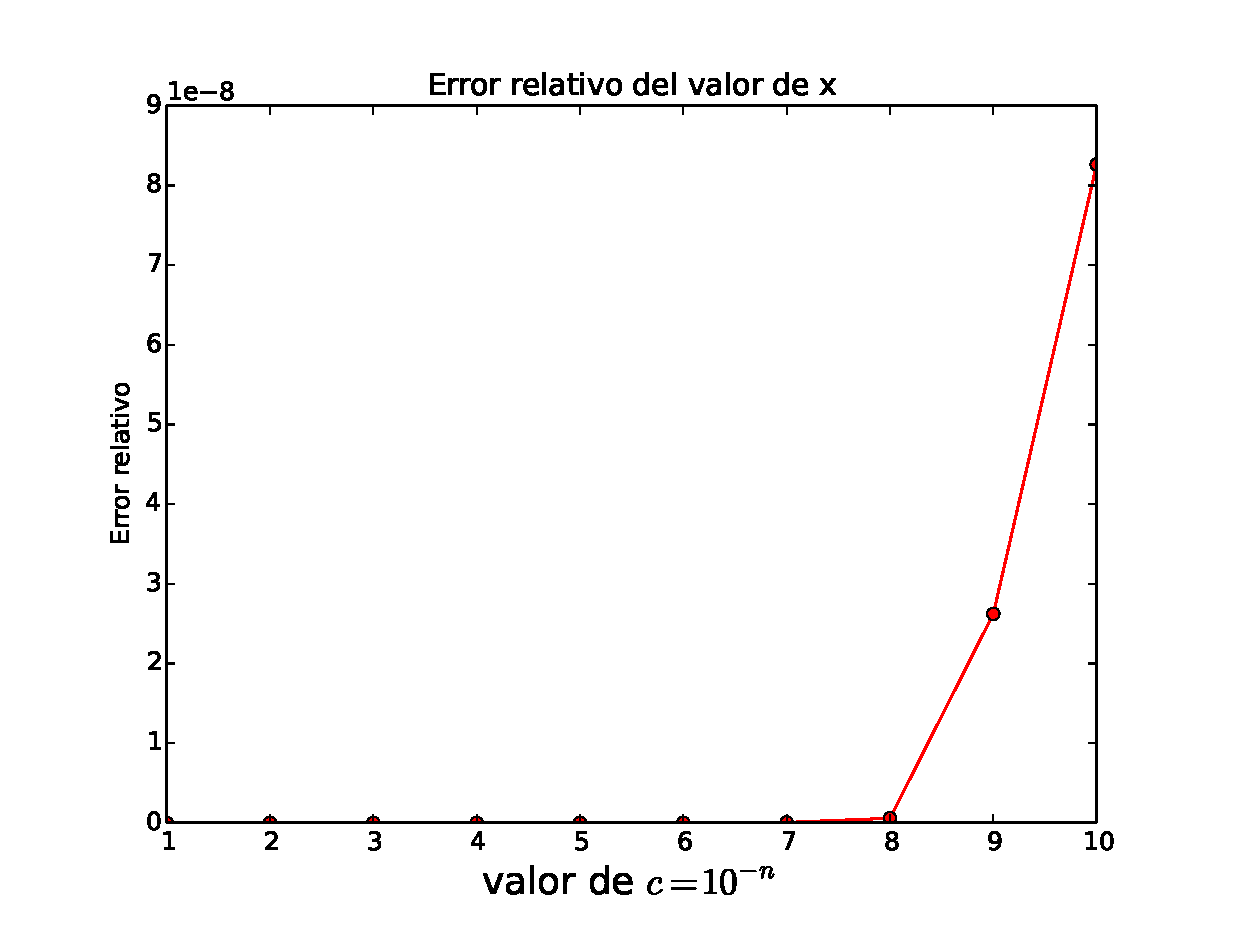
\includegraphics[scale=0.45]{Imagenes/Ejercicio_Eq_Cuadratica_01.eps} 
\end{figure}
\end{frame}
\begin{frame}
\frametitle{¿Qué estamos viendo?}
En la gráfica anterior, vemos una línea muy pegada al eje x, pero hay que considerar que el valor es muy pequeño, mientras que para $c=10^{-9}$, ya se eleva más el punto y se hace más notorio en la gráfica.
\\
\medskip
Podríamos pensar que el error relativo es casi el mismo para valores menores de $n=9$, pero hay que recordar que el ojímetro no funciona bien y menos en física computacional, por lo que ahora hacemos un cambio de escala en el eje y, para ello, usamos la función \texttt{semilogy()} de la librería \texttt{matplotlib}, que nos cambia la escala a una de tipo semilogarítmico.
\end{frame}
\begin{frame}[fragile]
\frametitle{Gráfica del error relativo y el valor de c, ajustando el eje y}
\begin{figure}
	\centering
	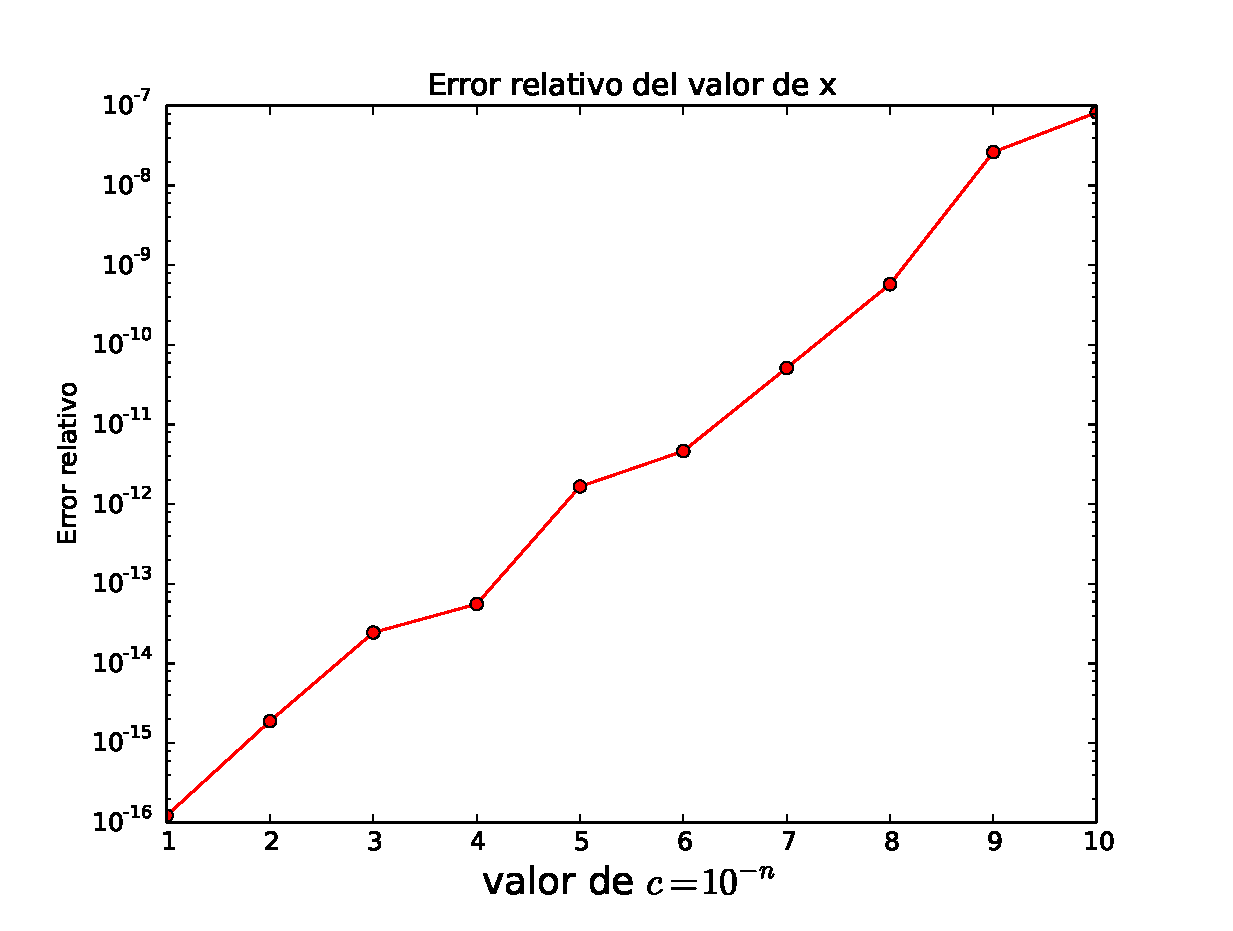
\includegraphics[scale=0.45]{Imagenes/Ejercicio_Eq_Cuadratica_02.eps} 
\end{figure}
\end{frame}
\begin{frame}
\frametitle{Tenemos una mejor idea de lo que ocurre}
\begin{itemize}
\item Vemos que existe una ''tendencia'' lineal (adviertiendo que uno de los ejes está en escala logarítmica)
\item El error relativo va aumentando conforme se incrementa el valor de $n$.
\item Hay algunas variaciones con respecto al valor de error, es decir, la dispersión es notaria, aunque no hemos dicho que debe de ser estrictamente un comportamiento lineal.
\item ¿Qué podemos hacer para evitar las operaciones entre valores muy grandes ($b=1$) con valores muy pequeños ($4ac$) ?
\end{itemize}
\end{frame}
\end{document}